% --------------------------------------------------------------
% This is all preamble stuff that you don't have to worry about.
% Head down to where it says "Start here"
% --------------------------------------------------------------

\documentclass[11pt]{article}

\usepackage[margin=1in]{geometry}
\usepackage{times}
\usepackage{amsmath,amsthm,amssymb}
\usepackage{caption}
\usepackage{graphicx,subfigure}
\usepackage{listings}
\usepackage{url}
\lstset{language=Pascal}

\newcommand{\N}{\mathbb{N}}
\newcommand{\Gauss}{\mathcal{N}}
\newcommand{\Z}{\mathbb{Z}}
\newcommand{\E}{\mathbb{E}}
\newcommand{\R}{\mathbb{R}}
\newcommand{\p}{{\bf p}}
\newcommand{\1}{\mathbf{1}}

\linespread{0}

\newenvironment{theorem}[2][Theorem]{\begin{trivlist}
\item[\hskip \labelsep {\bfseries #1}\hskip \labelsep {\bfseries #2.}]}{\end{trivlist}}
\newenvironment{lemma}[2][Lemma]{\begin{trivlist}
\item[\hskip \labelsep {\bfseries #1}\hskip \labelsep {\bfseries #2.}]}{\end{trivlist}}
\newenvironment{claim}[2][Claim]{\begin{trivlist}
\item[\hskip \labelsep {\bfseries #1}\hskip \labelsep {\bfseries #2.}]}{\end{trivlist}}
\newenvironment{exercise}[2][Exercise]{\begin{trivlist}
\item[\hskip \labelsep {\bfseries #1}\hskip \labelsep {\bfseries #2.}]}{\end{trivlist}}
\newenvironment{problem}[2][Problem]{\begin{trivlist}
\item[\hskip \labelsep {\bfseries #1}\hskip \labelsep {\bfseries #2.}]}{\end{trivlist}}
\newenvironment{question}[2][Question]{\begin{trivlist}
\item[\hskip \labelsep {\bfseries #1}\hskip \labelsep {\bfseries #2.}]}{\end{trivlist}}
\newenvironment{corollary}[2][Corollary]{\begin{trivlist}
\item[\hskip \labelsep {\bfseries #1}\hskip \labelsep {\bfseries #2.}]}{\end{trivlist}}

\begin{document}
{\raggedright

% --------------------------------------------------------------
%                         Start here
% --------------------------------------------------------------

\title{ECE 544NA HW2}%replace X with the appropriate number
\author{Jiaqi Mu~jiaqimu2 \\
collaborating with Hongyu Gong~hgong6 \\
[8pt]%replace with your name
Department of Electrical and Computer Engineering} %if necessary, replace with your course title

\maketitle

\section{Pencil-and-Paper\label{sec:1}}
In this part of the assignment, you will compute the derivatives/gradients and backpropped error for the following common modules in a neural network.

\begin{itemize}
\item {\bf Derivative of Softmax:} Recall the softmax function:
\begin{align*}
  \vec{y}[k] = \frac{e^{\vec{z}[k]}}{\sum_{l=1}^C e^{\vec{z}[l]}},
\end{align*}
what is $\frac{\partial \vec{y}[k]}{\partial z[j]}$.
\begin{proof}
  The derivative is given as follows,
  \begin{align*}
    \frac{\partial \vec{y}[k]}{\partial \vec{z}[j]} &= \frac{\partial}{\partial \vec{z}[j]} \frac{e^{{\vec{z}}[k]}}{\sum_{l=1}^C e^{{\vec{z}}[l]}} \\
    &=\frac{\sum_{l=1}^C e^{{\vec{z}}[l]} \frac{\partial}{\partial \vec{z}[j]} e^{\vec{z}[k]} - e^{\vec{z}[k]} \frac{\partial}{\partial \vec{z}[j]} \sum_{l=1}^C e^{{\vec{z}}[l]} }{\left(\sum_{l=1}^C e^{{\vec{z}}[l]}\right)^2} \\
    &= \frac{e^{\vec{z}[j]} \1_{j=k} \sum_{l=1}^C e^{{\vec{z}}[l]}  - e^{\vec{z}[k]} e^{\vec{z}[j]} }{\left(\sum_{l=1}^C e^{{\vec{z}}[l]}\right)^2} \\
    &= \frac{e^{\vec{z}[j]}\1_{j=k}}{\sum_{l=1}^C e^{{\vec{z}}[l]}} - \frac{e^{\vec{z}[k] + \vec{z}[j]}}{\left(\sum_{l=1}^C e^{{\vec{z}}[l]}\right)^2}.
  \end{align*}
\end{proof}
\item {\bf Negative Log Likelihood loss for Multi-class:} Recall the negative log likelihood,
\begin{align*}
  L = -\sum_{i}^N \sum_k^K \1_{y_i =k} \log (\hat{\vec{y}}_i[k]).
\end{align*}
What is $\frac{\partial L}{\partial \hat{\vec{y}}_i[j]}$.
\begin{proof}
  The derivative is given as follows (here we take the $\log$ as natural logarithm),
  \begin{align*}
    \frac{\partial L}{\partial \hat{\vec{y}}_i[j]} &= -\sum_{i}^N \sum_k^K \1_{y_i =k} \frac{\partial}{\partial \hat{\vec{y}}_i[j]} \log (\hat{\vec{y}}_i[k]) \\
    &= -\sum_{i}^N \sum_k^K \1_{y_i =k} \1_{k = j} \frac{1}{\hat{\vec{y}}_i[j]} \\
    &= -\sum_{i}^N \1_{y_i =j} \frac{1}{\hat{\vec{y}}_i[j]}
  \end{align*}
\end{proof}
\item {\bf Avg-pooling (1D):} Revall Avg-pooling operation with window size $W$:
\begin{align*}
  \vec{y}[i] = \frac{1}{W} \sum_{k=0}^{W-1} \vec{x}[i+k].
\end{align*}
What is $\frac{\partial \vec{y}[i]}{\partial \vec{x}[j]}$.
\begin{proof}
  The derivative is given as follows,
  \begin{align*}
    \frac{\partial \vec{y}[i]}{\partial \vec{x}[j]} &= \frac{1}{W} \sum_{k=0}^{W-1} \frac{\partial}{\partial \vec{x}[j]} \vec{x}[i+k] \\
    &= \frac{1}{W} \1_{i \le j < i+W}
  \end{align*}
\end{proof}
\item {\bf Max-pooling (1D):} Recall max-pooling (1D) operation with window size $W$:
\begin{align*}
  \vec{y}[i] = \max_{k=0}^{W-1} \vec{x}[i+k].
\end{align*}
What is $\frac{\partial \vec{y}[i]}{\partial \vec{x}[j]}$.
\begin{proof}
  The derivative is given as follows,
  \begin{align*}
    \frac{\partial \vec{y}[i]}{\partial \vec{x}[j]} &= \1_{j = i + \arg\max_{k=0}^{W-1} \vec{x}[i+k]}
  \end{align*}
\end{proof}
\item {\bf Convolutional layer (1D):} Recall Convolution (1D) operation, assume $\vec{w}$ is length 3, and zero index at the center:
    \begin{align*}
      \vec{y}[i] = (\vec{w} \star \vec{x})[i] = \sum_{k=-1}^1 \vec{x}[i-k] \vec{w}[k].
    \end{align*}
What is $\frac{\partial \vec{y}[i]}{\partial \vec{x}[j]}$? What is $\frac{\partial \vec{y}[i]}{\partial \vec{w}[j]}$?
\begin{proof}
  The derivatives are given as follow,
  \begin{align*}
    \frac{\partial \vec{y}[i]}{\partial \vec{x}[j]} &= \sum_{k=-1}^1 \frac{\partial}{\partial \vec{x}[j]} \vec{x}[i-k] \vec{w}[k] \\
    &= \sum_{k=-1}^1 \vec{w}[k] \1_{i-k = j} \\
    \frac{\partial \vec{y}[i]}{\partial \vec{w}[j]} &= \sum_{k=-1}^1 \frac{\partial}{\partial \vec{w}[j]} \vec{x}[i-k] \vec{w}[k] \\
    &= \vec{x}[i-j]\1_{-1 \le j \le 1}.
  \end{align*}
\end{proof}
\end{itemize}

\section{Code-From-Scratch}
Perform 9-way classification among the 9 letters in the ee-set using a fully-connected neural network with 2 hidden layers. Use the first 70 frames of each example and drop any example that is shorter than 70 frames. The use mini-batch gradient descent for optimization, you can pick the batch size. The test set accuracy is in the range of 35\% to 50\%.
\begin{itemize}
  \item Experiment with different number of hidden-nodes, \{10, 50\}, assume the two hidden layers have the same size.
  \item Experiment with different type of nonlinearities [sigmoid, tanh, relu]
\end{itemize}
\subsection{Methods}
\begin{itemize}
  \item Describe the functions you wrote, and the overall structure of your code.
  \begin{proof}
    The feedforward neural network is implemented as a class FNN in {\tt fnn.py}. This contains five functions:
    \begin{itemize}
      \item {\tt \_\_init\_\_:} initialize all hyperparameters, all weight matrices and biases.
      \item {\tt gradient:} compute the gradient of activation nonlinear functions.
      \item {\tt activation:} compute the activation nonlinear functions.
      \item {\tt train:} train the model using training data. This function can be divided into three parts: (a) feedforward, (b) back-propagation and (c) gradient update. 
      \item {\tt test:} test new instances.
    \end{itemize}
    The overall structure of my code is,
    \begin{itemize}
      \item First read data from training/dev/testing files.
      \item Initialize FNN model.
      \item Train FNN model.
      \item Test FNN model.
    \end{itemize}
  \end{proof}
  \item Describe the model architecture and specific hyperparameter you have chosen.
  \begin{proof}
    The model is compatible with hidden layers of size $N_{h_1}, N_{h_2},...,N_{h_K}$, where we choose $K=2$, and $N_{h_1} = N_{h_2} \in \{10, 50\}$ as a special case. The input dimension is $N_i = 16\times70$, the output dimension is $N_o = 9$. 

    In our case we choose step size to be {\tt 1e-2}, the number of iterations to be 100,000, batch size to be 50.
  \end{proof}
  \item Report the total number of weights in the models.
  \begin{proof}
    Thus the total number of weights in this model is,
    \begin{align*}
      {\rm weight matrix:} \qquad & N_i\times N_{h_1} + \sum_{k=1}^{K-1} N_{h_k} \times N_{h_{k+1}} + N_{K} \times N_o \\
      {\rm bias:} \qquad  & \sum_{k=1}^K N_{h_k} + N_o
    \end{align*}
    In our case, the number of parameters are listed in Table~\ref{tb:part2:parameters}.
    \begin{table}[htb]
    \centering
    \begin{tabular}{r|l|l}
    \hline
    hidden layer & weight matrix & bias \\
    \hline
    10 & 11390 & 29 \\
    \hline
    50 & 58950 & 109 \\
    \hline
    \end{tabular}
    \caption{The total number of parameters. \label{tb:part2:parameters}}
    \end{table}
  \end{proof}
\end{itemize}
\subsection{Results}
\begin{itemize}
  \item Report training and testing accuracy for your best model.
  \begin{proof}
    The best model in terms of development set is {\tt tanh} + hidden layer = 50. The accuracies are 100.00\% and 42.79\% for training and testing respectively. This is because of overfitting. 
  \end{proof}{}
  \item Report training and testing accuracy for all the models. (All combinations between nonlinearities and number of hidden nodes.)
  \begin{proof}
    The accuracies are given in Table~\ref{tb:part2:2}. 
    \begin{table}[htbp]
    \centering{}
    \begin{tabular}{c|c|c|c|c|c|c}
    \hline
    Accuracy & \multicolumn{3}{c|}{hidden layer size = 10} & \multicolumn{3}{c}{hidden layer size = 50} \\ \cline{2-7}
     & sigmoid & tanh & relu & sigmoid & tanh & relu \\ \hline
    Training & 80.01 & 78.74 &  71.66 & 100.0 & 100.0 & 100.0 \\ \hline
    Development & 44.46 & 39.81 &  43.50  & 46.79 & \bf 48.42* & 48.29 \\ \hline
    Testing & 39.60 & 37.62 & 38.94 & 38.28 & 42.79 & 45.87 \\ \hline
    \end{tabular}
    \caption{Training and testing Accuracy (x100)}
    \label{tb:part2:2}
    \end{table}
  \end{proof}
  \item Report the running time (in seconds) for one iteration of backpropagation on model with 10 and 50 hidden-nodes. Also describe how the runng time varies with batch size.
  \begin{proof}
    The running time is given in Figure~\ref{fig:part2:3}. We can observe the running time almost grows linearly with the batch size.
    \begin{figure}[htbp]
    \centering
    \subfigure[\tt reLu]
    {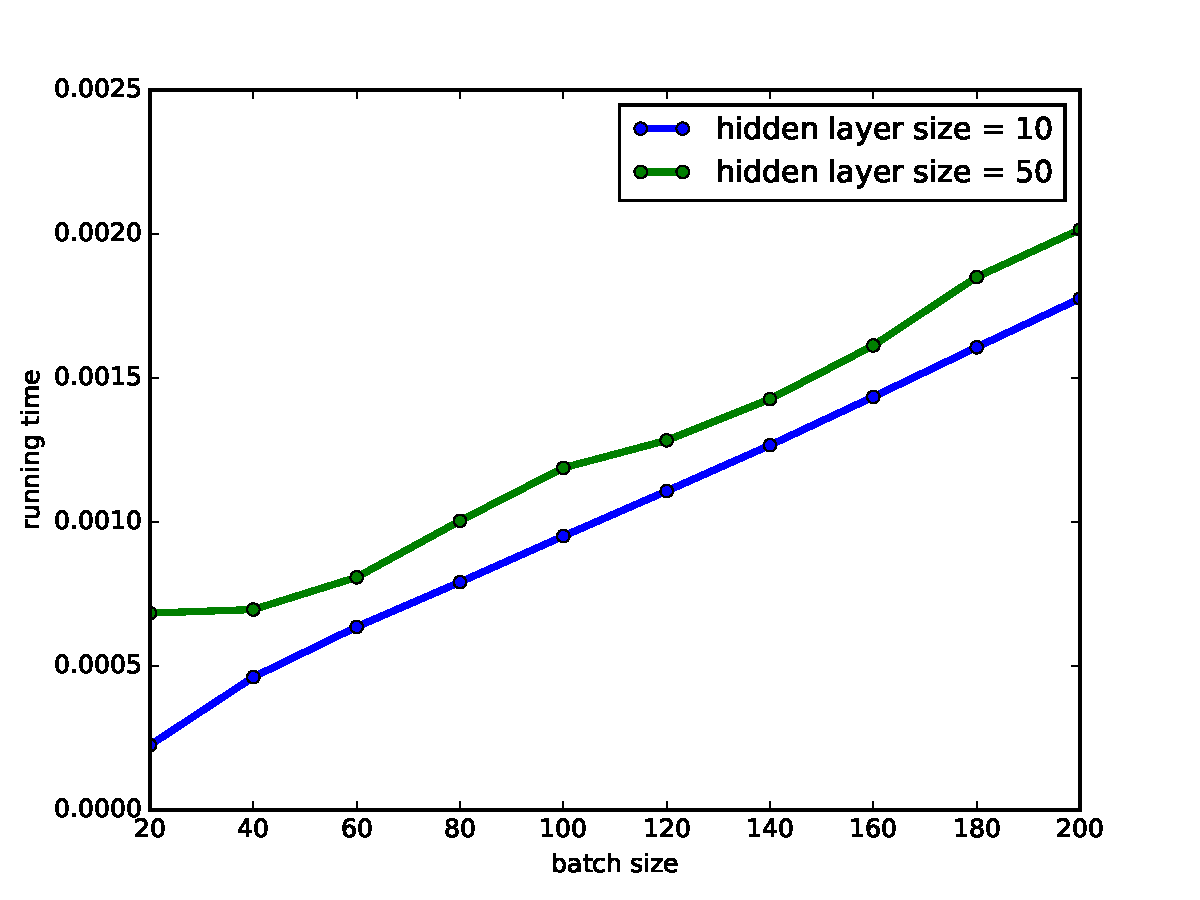
\includegraphics[width=0.3\textwidth]{../figures/relu-running-time.pdf}}
    \subfigure[\tt tanh]
    {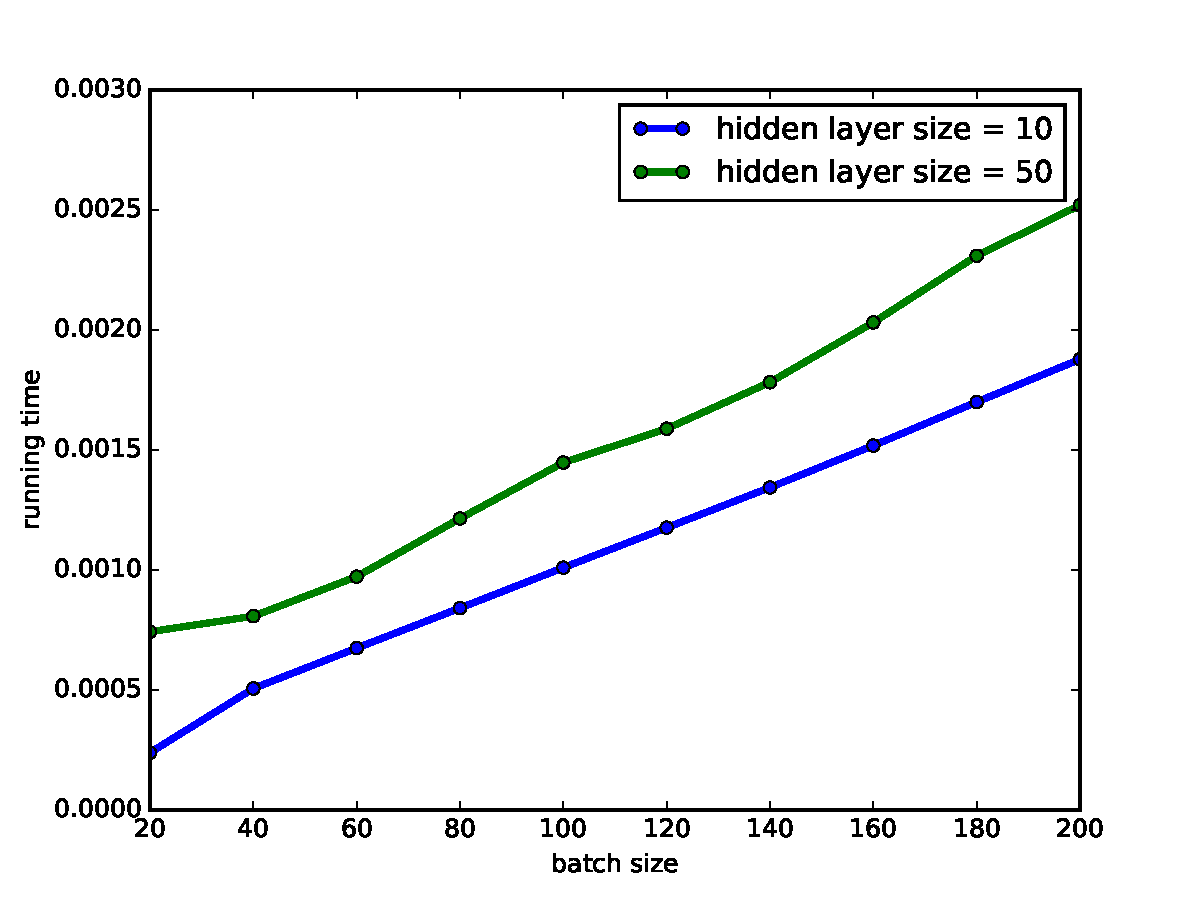
\includegraphics[width=0.3\textwidth]{../figures/tanh-running-time.pdf}}
    \subfigure[\tt sigmoid]
    {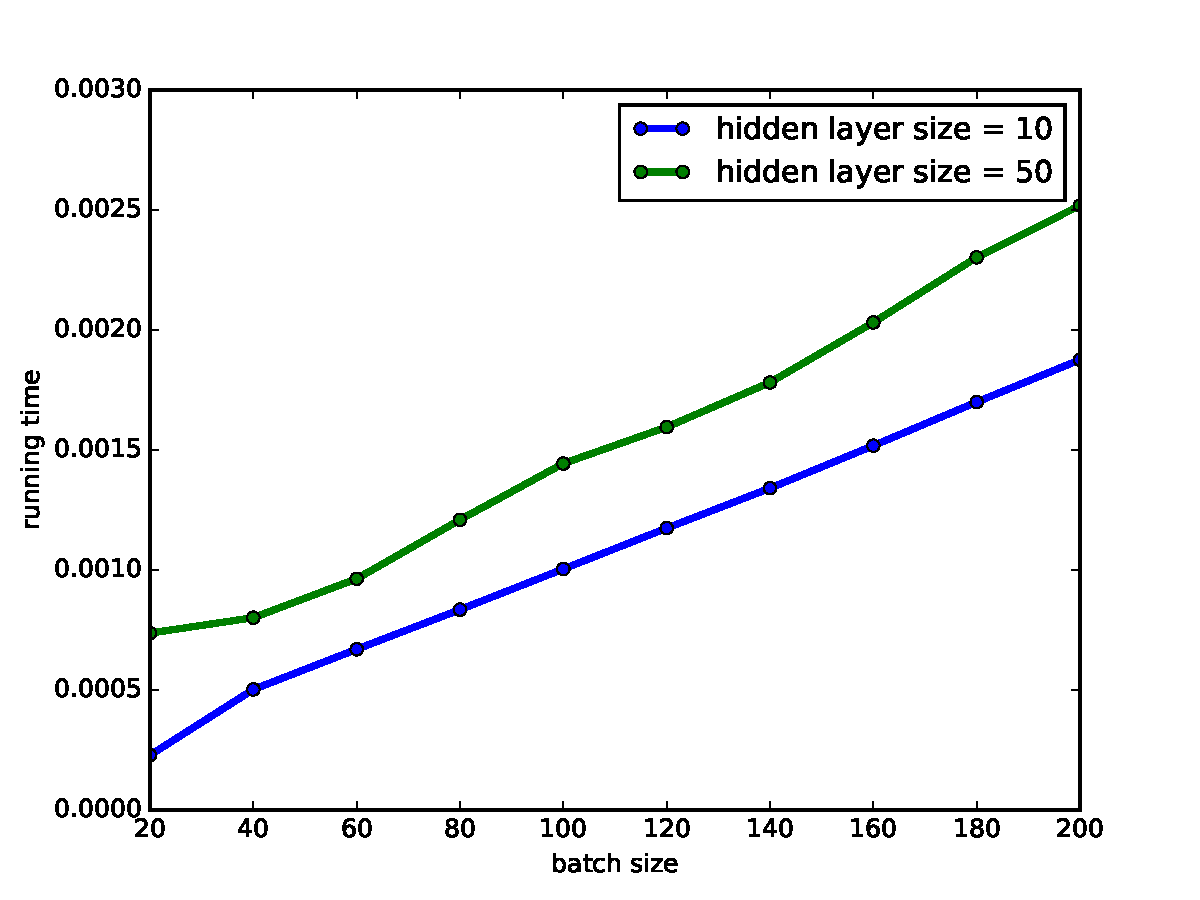
\includegraphics[width=0.3\textwidth]{../figures/sigmoid-running-time.pdf}}
    \caption{Running time versus batch sizes. \label{fig:part2:3}}
    \end{figure}
  \end{proof}
  \item Plot training and testing classification confusion matrix for your best model.
  \begin{proof}
    The training and testing confusion matrix for the best model described in part 2 is given in Figure \ref{fig:part2:4}.
    \begin{figure}[htbp]
    \centering
    \subfigure[train]
    {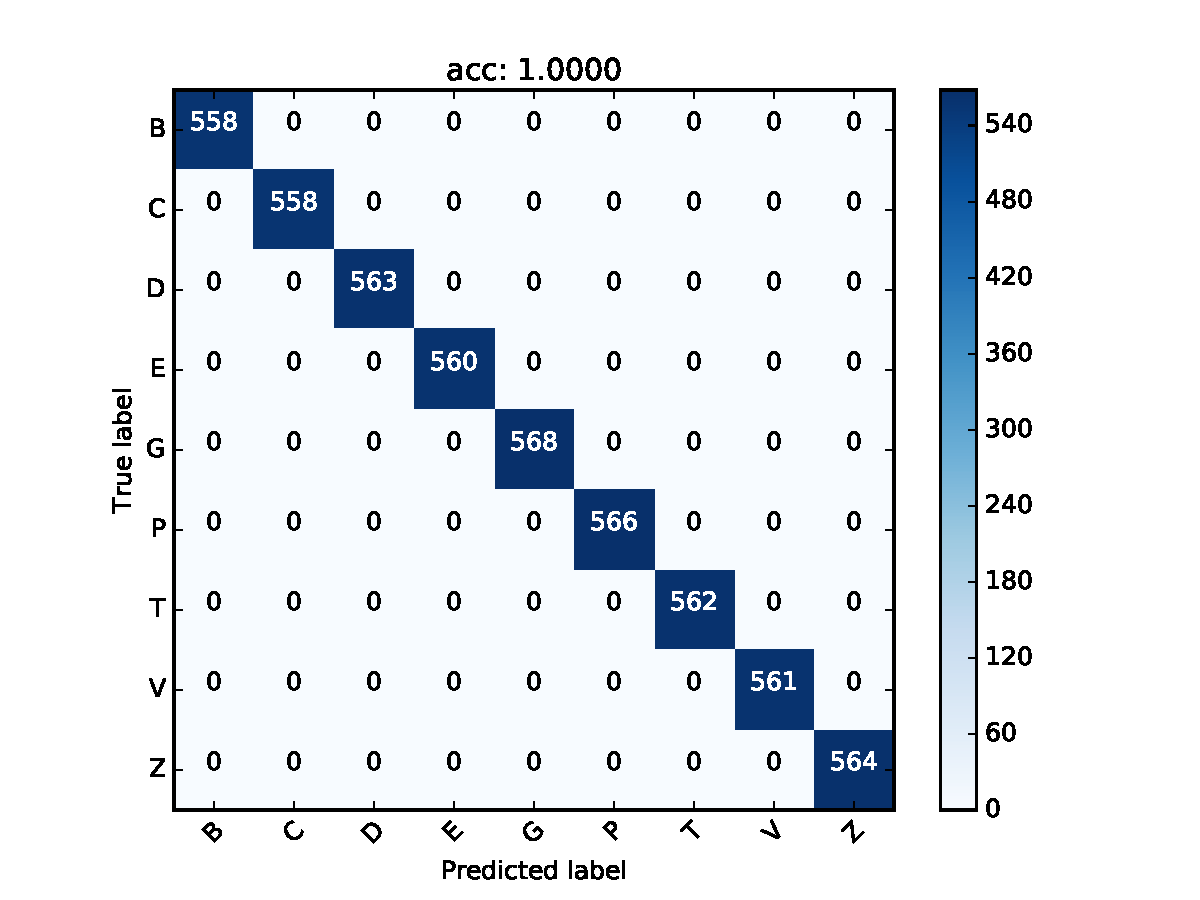
\includegraphics[width=0.4\textwidth]{../figures/tanh-50-train-conf-matrix.pdf}}
    \subfigure[test]
    {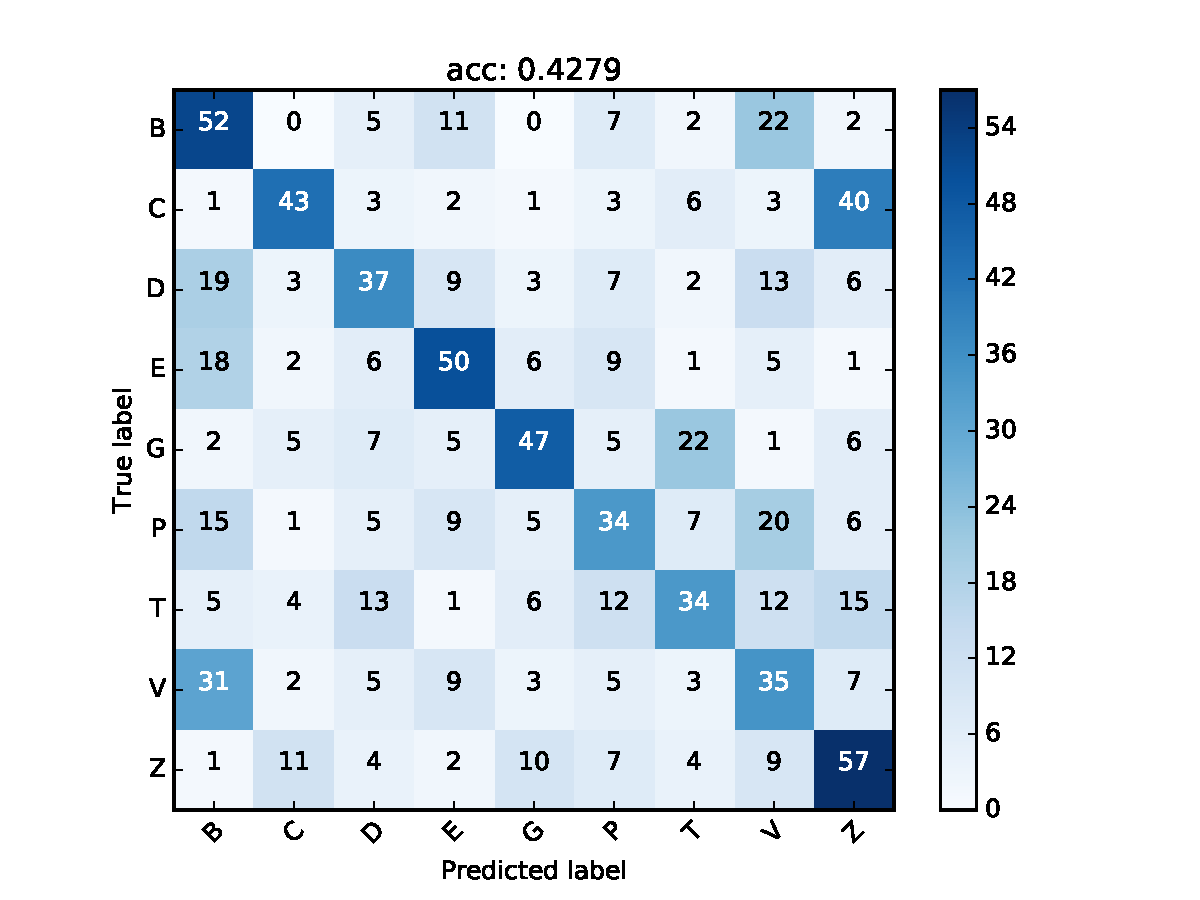
\includegraphics[width=0.4\textwidth]{../figures/tanh-50-test-conf-matrix.pdf}}
    \caption{Confusion matrix. \label{fig:part2:3}}
    \end{figure}
  \end{proof}
\end{itemize}

\section{TensorFlow}
Perform 9-way classification among the 9 letters in the ee-set using the TDNN architecture of Waibel, Hanazawa, Hinton, Shikano and Lang\footnote{\url{http://ieeexplore.ieee.org/document/21701/?arnumber=21701&tag=1}}. Use the first 70 frames of each example and drop any example that is shorter than 70 frames. The use mini-batch gradient descent for optimization, you can pick the batch size. The test set accuracy is in the range of 35\% to 50\%.

Use the following network architecture:
Input layer: ($J$=16, $N$=2), Hidden Layer 1: ($J$=8, $N$=4), Hidden Layer 2: ($J$=3, $N$=1), Final Layer: multi-class logistic regression.

Next, try changing the TDNN architecture or even CNN architecture and see if you can improve the accuracy (The accuracy for this part will not affect your grade) Here is a TensorFlow tutorial
\footnote{\url{https://www.tensorflow.org/versions/r0.10/tutorials/mnist/pros/index.html}} with CNN on the MNIST datase.

\subsection{Metods}
\begin{itemize}
  \item Describe the TDNN architecture, and discuss how you used TensorFlow functions to create such architecture.
      \begin{proof}
        For simplicity, we ignore the index for sample. We denote the input layer as $h^0$, the first hidden layer as $h^1$, the second hidden layer as $h^2$, and the output multi-class logistic regression as $\hat{y}$. Here we know that $h^0 \in \R^{16\times 70}$, $h^1 \in \R^{8\times 68}$, $h^2 \in \R^{3 \times 64}$, and $\hat{y} \in \R^9$. The dependencies are as follow,
        \begin{align}
          h^1_t &= f_1\left(\sum_{\tau = 0}^2 W^1_\tau h^0_{t+\tau} + b^1\right), t=1,2,...,68 \label{eq:hidden1}\\
          h^2_t &= f_2\left(\sum_{\tau = 0}^4 W^2_\tau h^1_{t+\tau} + b^2\right), t=1,2,...,64 \label{eq:hidden2}\\
        \end{align}
        where the subscript $t$ indicates the time frame,  $W^1_{\tau} \in \R^{8\times 16}$, $b^1 \in \R^8$,  $W^2_{\tau} \in \R^{3\times 8}$, $b^2 \in \R^3$ and $f_1$ and $f_2$ are non-linear kernels. The output $\hat{y}$ is computed via a multi-class softmax, where $\vec{y}$ is computed via,
        \begin{align}
          \vec{y} = {\rm softmax}\left(W^3 \sum_{t=1}^{64} h_t^2 + b^3\right), \label{eq:output}
        \end{align}
        where $W^3 \in \R^{9\times 3}$ and $b^3 \in \R^9$.

        We can achieve this architecture using the built-in convolutional network module from TensorFlow. Specific functions are as follow:
        \begin{itemize}
          \item Initialization of weight matrices through {\tt weight\_variable(shape)}, which uses {\tt tf.truncated\_normal} to randomly generated weight matrices.
          \item Initialization of bias vectors through {\tt bias\_variable(shape)}, which uses {\tt tf.constant} to generate bias vectors.
          \item Convolution layer through {\tt tf.nn.conv2d(z, W, stride=[1,1,1,1], padding=`VALID')} where we set the stride size to be 1, and the padding size to be `{\tt VALID}' meaning we do not pad zeros on the boundary. Note here:
          \begin{itemize}
          \item {\tt z} denotes for $h^0$, $h^1$, and $h^2$, and has to be reshaped into $[-1,T_l,1,J_l]$, where $T_l$ is the number of total frames, and $J_l$ is the number of units/channels in $l$-th layer.
          \item {\tt W} denotes the weight matrix associated with {\tt z}, and should be shaped as $[N_l+1, 1, J_l, J_{l+1}]$.
          \end{itemize}
          \item Activation layer though ReLU/Sigmoid by calling {\tt tf.nn.relu}/{\tt tf.sigmoid}.
          \item Softmax layer though {\tt tf.nn.softmax} as seen in HW1.
        \end{itemize}
      \end{proof}
  \item Describe the variations of the TDNN architecture you have tried and anything interesting.
  \begin{proof}
    Apart from this architecture, we use a different output layer. We first reshape $h^2$ into a vector, and directly apply a weighted softmax on that. Note this is a generalization to \eqref{eq:output}.
  \end{proof}
  \item Report the total number of weights in the original TDNN architecture.
  \begin{proof}
    The number of weights in the first layer is 384(=8x16x3), the number of weights in the second layer is 120(=5x3x8), and the number of weights in the output layer is 27(=9x3). The number of biases in the first layer is 8, that in the second layer is 3, and that in the output layer is 9.
  \end{proof}
  \item Report the activation dimensions at each layer.
  \begin{proof}
    The activation dimension at the first hidden layer is 8, that at the second hidden layer is 3.
  \end{proof}
  \item Discuss which Tensorflow functions you used, and how. Additionally, explain the overall organization/structure of your code, you should refer to specific part of your code.
  \begin{proof}
    The functions are listed in part 1. Details of the code organization is as follows:
    \begin{itemize}
      \item {\tt data.py} is a class storing training samples, development samples, and test samples. Two functions are involved in this class:
          \begin{itemize}
            \item {\tt readFile(filename)} is to read data from files.
            \item {\tt nextBatch(batchSize)} is to get the next batch for training, specially when {\tt batchSize=}-1 return all samples.
          \end{itemize}
      \item {\tt part3.py} is the main script for TDNN.
      \begin{itemize}
        \item Line 36-38: set up train/dev/test data;
        \item Line 48-51: preprocess samples (i.e., reshape them into proper dimensions);
        \item Line 56-61: compute the first hidden layer;
        \item Line 66-71: compute the second hidden layer;
        \item Line 76-85: compute the output;
        \item Line 90: specify the objective loss function;
        \item Line 93: set up the gradient descent;
        \item Line 94-95: set up the evaluation metric;
        \item Line 99-106: execute the training model.
      \end{itemize}
    \end{itemize}
  \end{proof}
\end{itemize}

\subsection{Results}
The hyperparameters are as follow: step size: 1e-3 for {\tt AdamOptimizer}; batch size: 50; iterations: 100,000 for softmax and 10,000 for reLu.

\begin{itemize}
  \item Report training and testing accuracy for the TDNN model.
      \begin{proof}
        The accuracy for the original TDNN structure with two different nonlinear filters is reported in Table~\ref{tf:acc1}.
        \begin{table}[htbp]
        \centering
          \begin{tabular}{r|l|l|l}
          \hline
            & train & test & dev\\
            \hline
            {\tt sigmoid} & 50.19 & 38.72 & 47.20 \\
            \hline
            {\tt reLu} & 43.18 & 37.07 & 40.77\\
            \hline
          \end{tabular}
          \caption{Training and testing accuracy of original TDNN (x100).\label{tf:acc1}}
        \end{table}
      \end{proof}
  \item Report training and testing accuracy for your best model.
      \begin{proof}
        We flatten the hidden layer to feed in a fully-connected feedforward neural network. The accuracies are in Table~\ref{tf:acc1}. The best one is a FNN+reLu.
        \begin{table}[htbp]
        \centering
          \begin{tabular}{r|l|l|l}
          \hline
            & train & test & dev \\
            \hline
            {\tt sigmoid} & 68.34 & 44.22 & \bf 52.12*\\
            \hline
            {\tt reLu} & 61.91 & 47.63 & 49.79\\
            \hline
          \end{tabular}
          \caption{Training and testing accuracy of modified TDNN (x100).\label{tf:acc1}}
        \end{table}
      \end{proof}
  \item Plot training and testing classification confusion matrix for the TDNN model, and your best model.
      \begin{proof}
        The confusion matrices are reported in Figure~\ref{tf:confmat}, where (a) and (b) are for TDNN with sigmoid activation, (c) and (d) are for TDNN with relu activation, and (e) and (f) are for the best model.
        \begin{figure}[htbp]
          \centering
          \subfigure[TDNN-sigmoid-train]
          {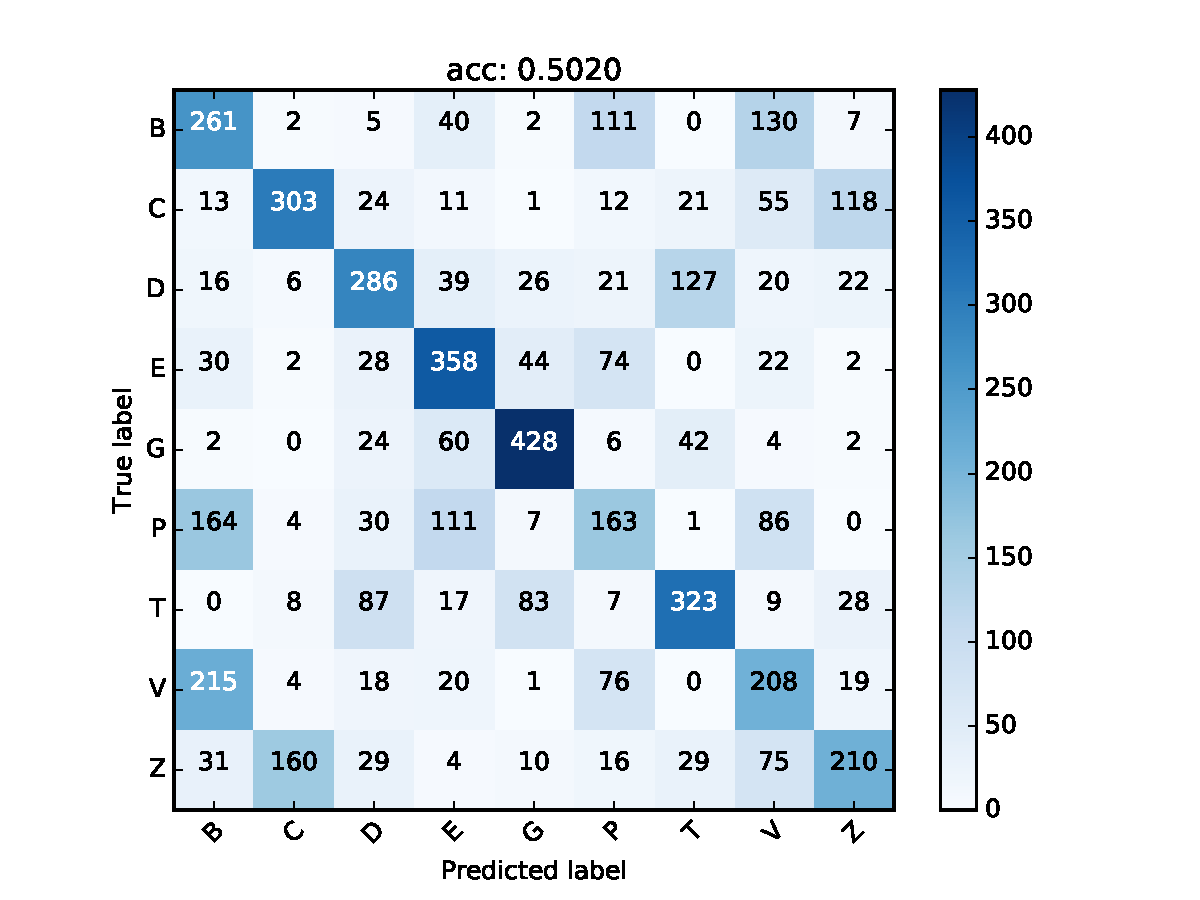
\includegraphics[width=0.4\textwidth]{../figures/sigmoid-sum-train.pdf}}
          \subfigure[TDNN-sigmoid-test]
          {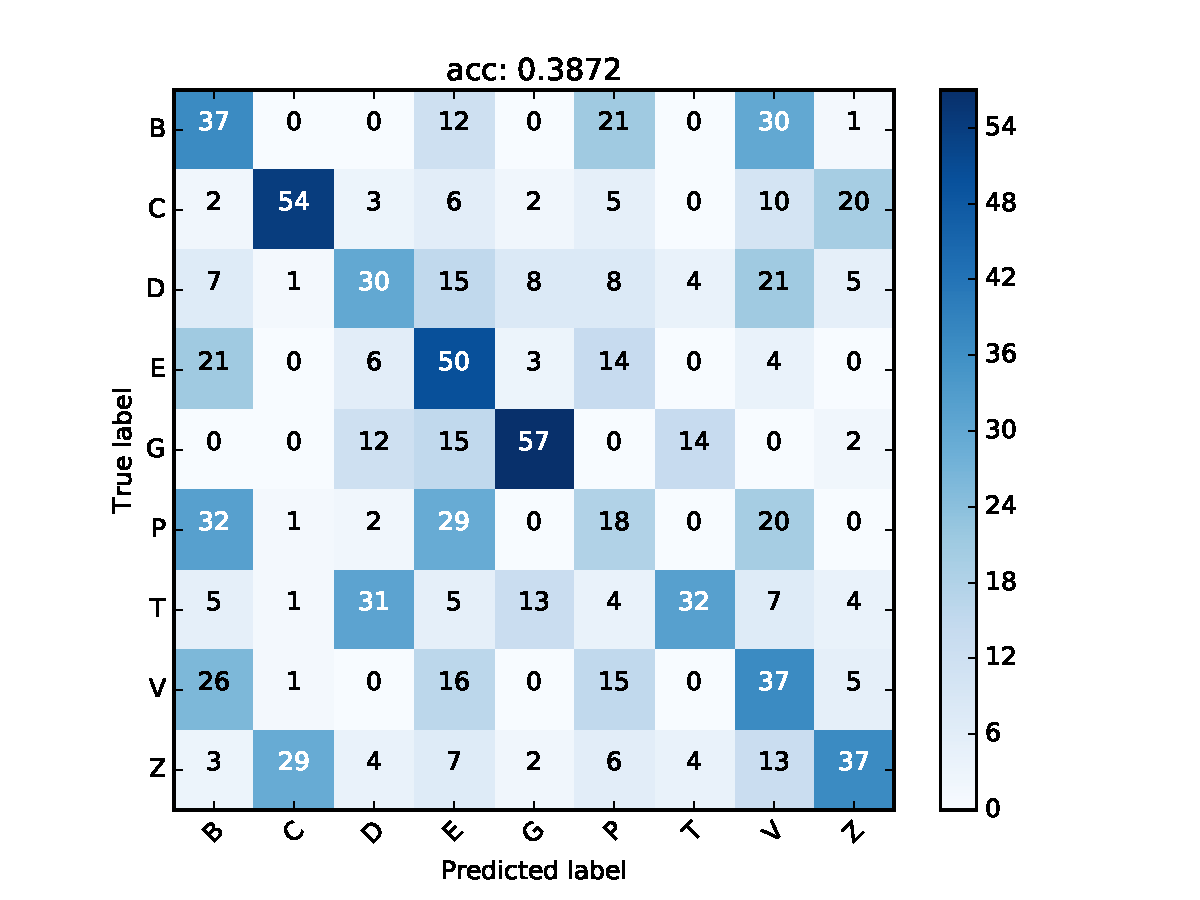
\includegraphics[width=0.4\textwidth]{../figures/sigmoid-sum-test.pdf}}
          \subfigure[TDNN-reLu-train]
          {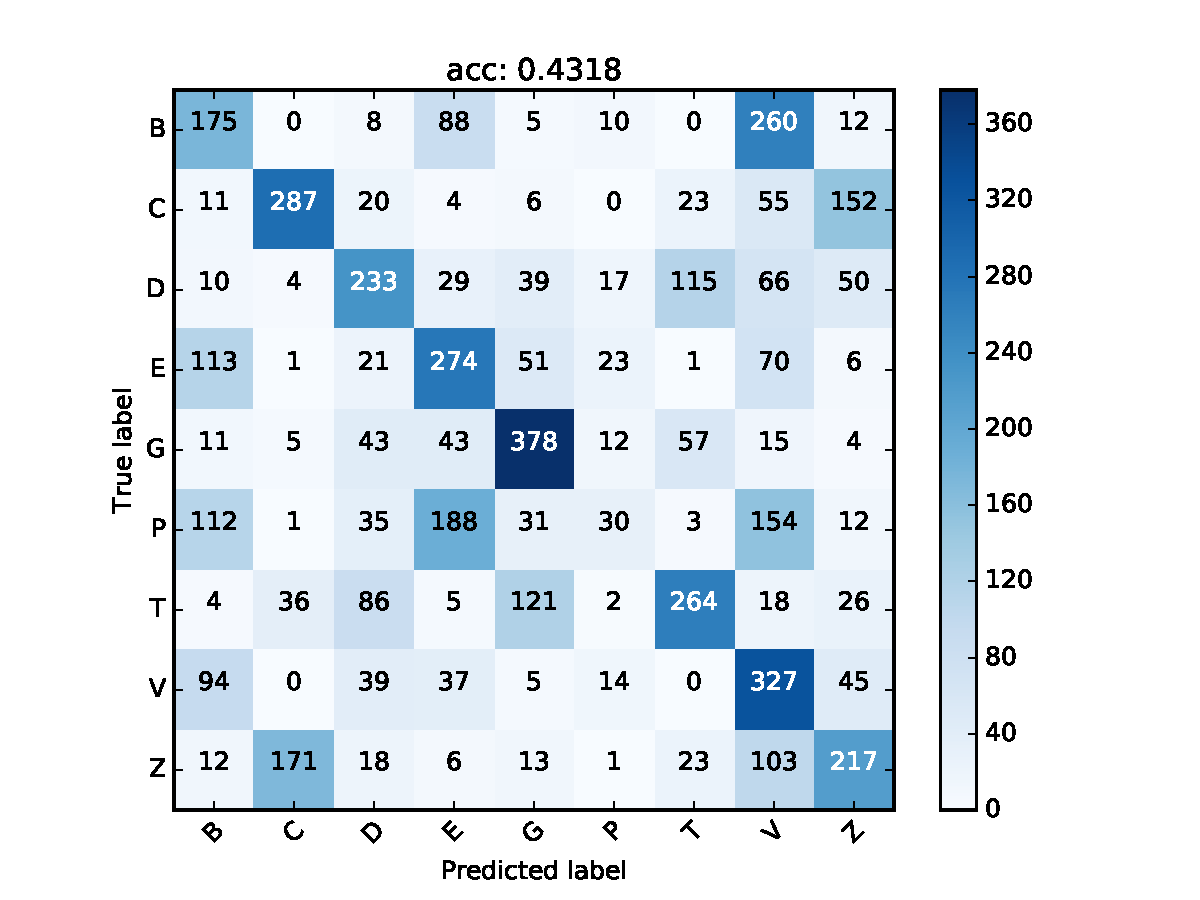
\includegraphics[width=0.4\textwidth]{../figures/relu-sum-train.pdf}}
          \subfigure[TDNN-reLu-test]
          {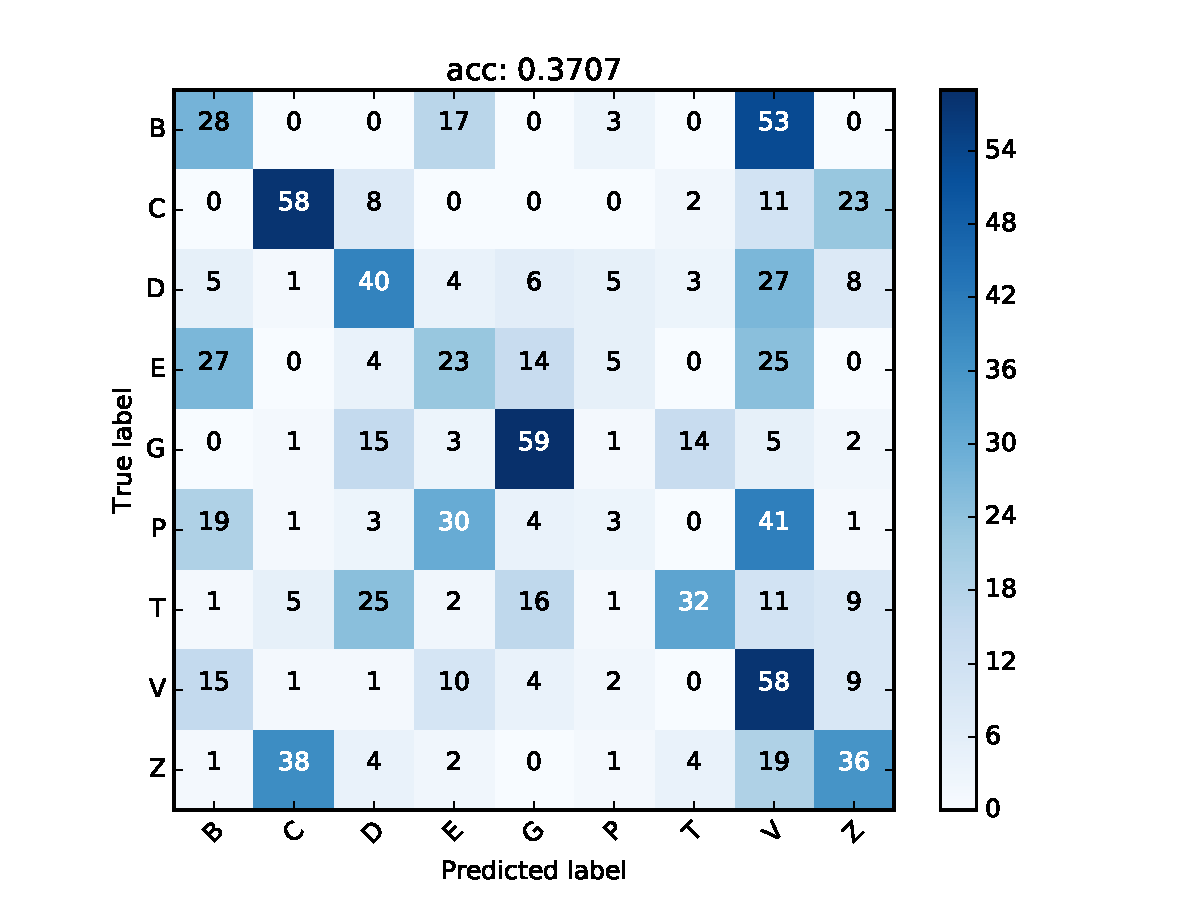
\includegraphics[width=0.4\textwidth]{../figures/relu-sum-test.pdf}}
          \subfigure[best model-train]
          {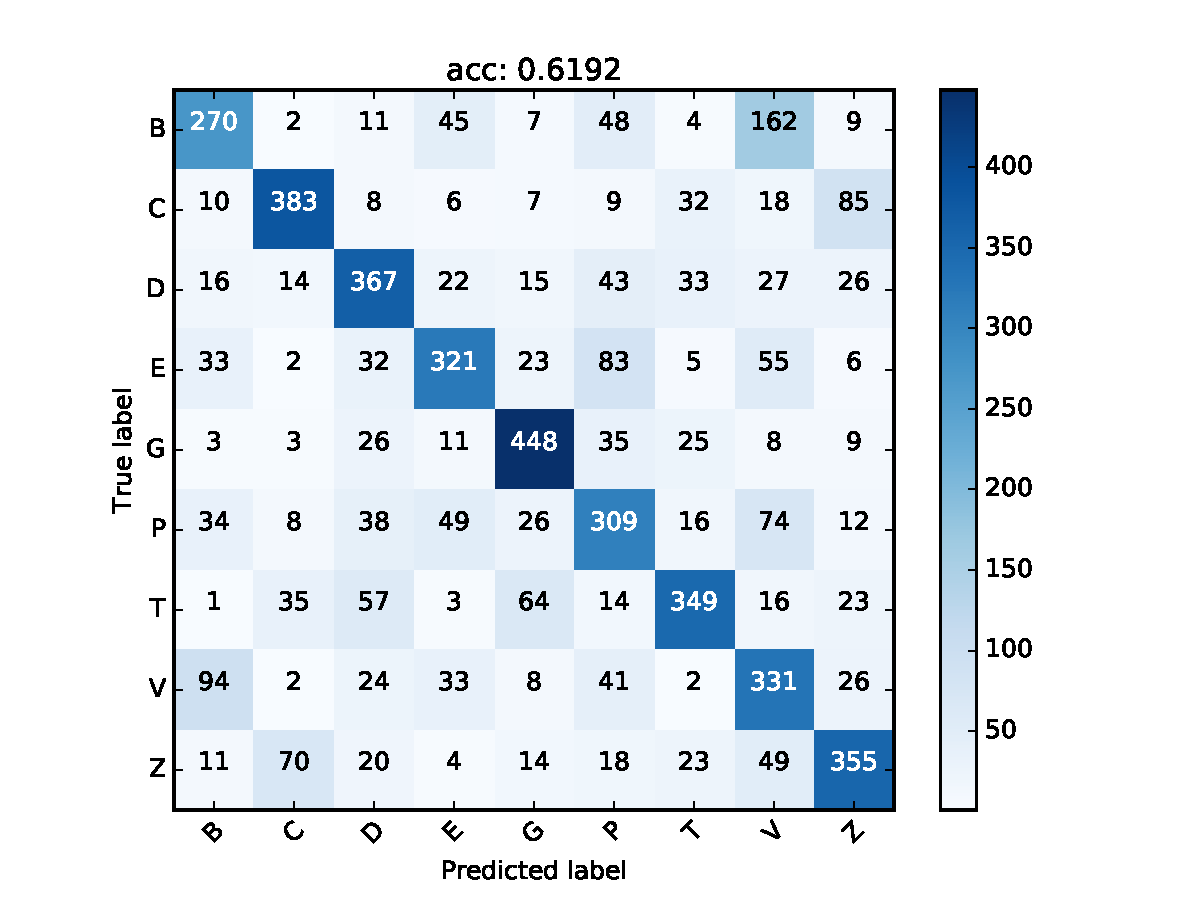
\includegraphics[width=0.4\textwidth]{../figures/relu-fnn-train.pdf}}
          \subfigure[best model-test]
          {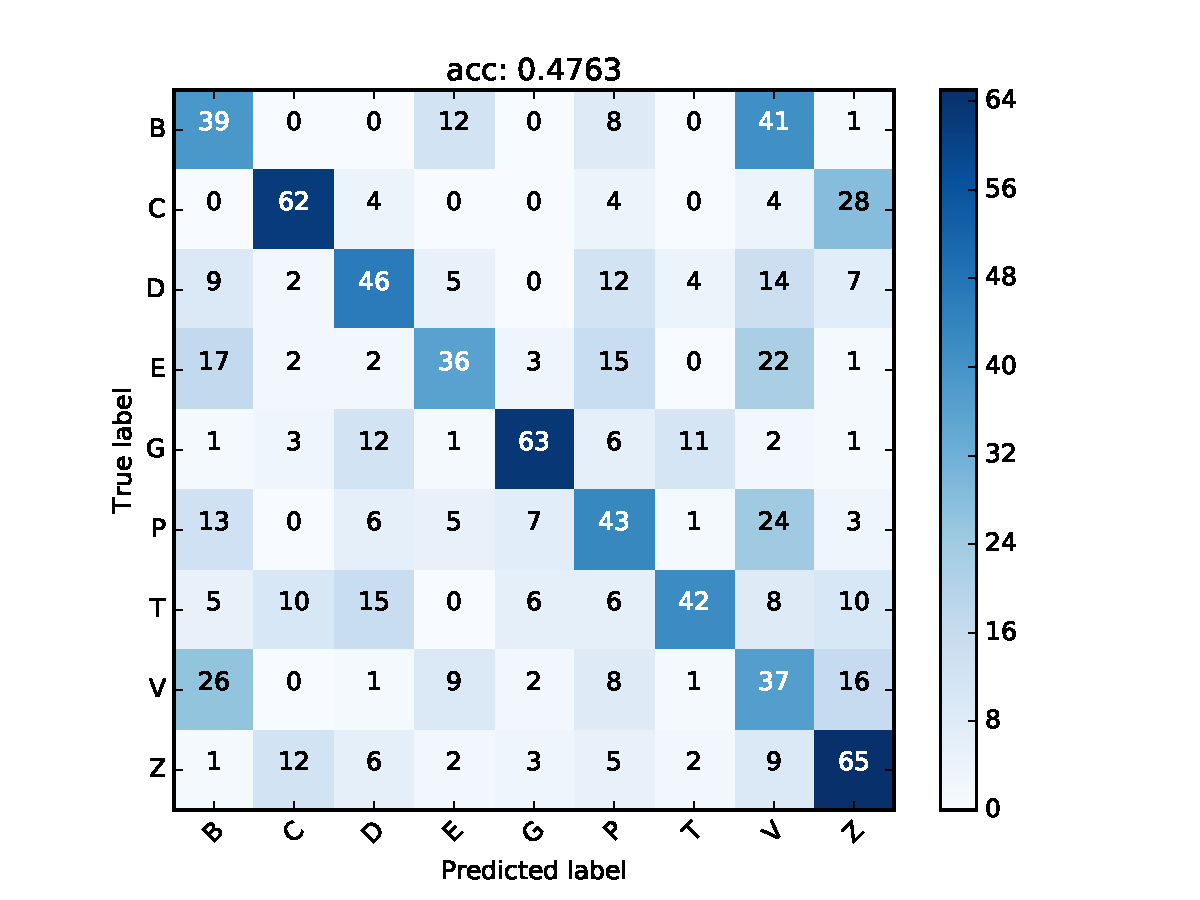
\includegraphics[width=0.4\textwidth]{../figures/relu-fnn-test.pdf}}
          \caption{Confusion matrix.\label{tf:confmat}}
        \end{figure}
      \end{proof}
\end{itemize}

\par}
\end{document}
